\section{Creación de un Data Source View} 

En el Solution Explorer nos ubicamos en Data Sources View y click derecho, seleccionando la opción de
New Data Source View …
	\begin{center}
	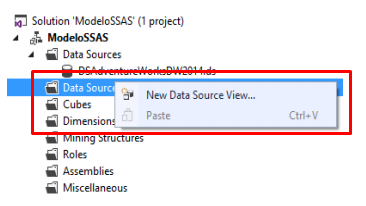
\includegraphics[width=8cm]{images/task2/img9}
	\end{center}	

Se nos abrirá una ventana de resumen. Click en Next:
\begin{center}
	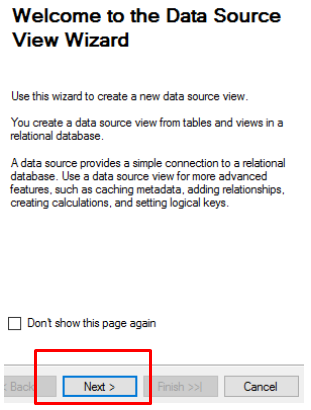
\includegraphics[width=8cm]{images/task2/img10}
\end{center}
Aquí nos aparecerán todos los Data Sources creados en la proyecto, en mi caso nos aparece el creado en
la sección 1. Click en Next:

\begin{center}
	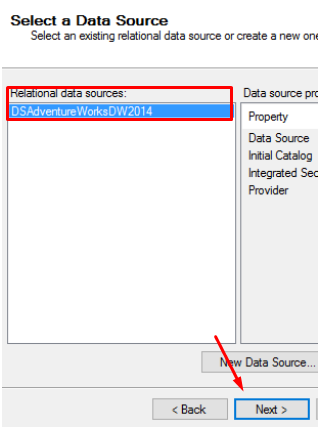
\includegraphics[width=8cm]{images/task2/img11}
\end{center}
Si bien es cierto hemos creado una conexión hacia Adventure Works DW, solo trabajaremos con algunas
tablas. Seleccionamos las tablas DimDate,DimProduct y FactInternetSales:
\begin{center}
	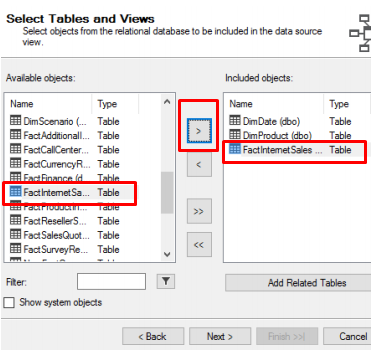
\includegraphics[width=8cm]{images/task2/img12}
\end{center}
Click en Next.
Colocamos un nombre el Data Source View creado y click en Finish:
\begin{center}
	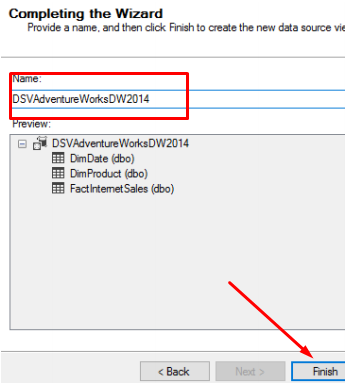
\includegraphics[width=8cm]{images/task2/img13}
\end{center}
Si todo va bien visualizaremos las tablas seleccionadas en el Data Source View:
\begin{center}
	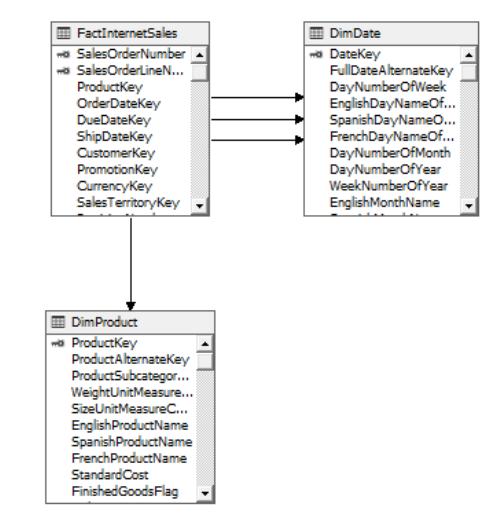
\includegraphics[width=8cm]{images/task2/img14}
\end{center}